\question{Câu 4}

Cho mạch khuếch đại tín hiệu như hình vẽ. Giả sử các tụ có giá trị rất lớn. BJT có $\beta = 100$ và $V_{A} = \infty$.

\begin{figure}[H]
	\centering
	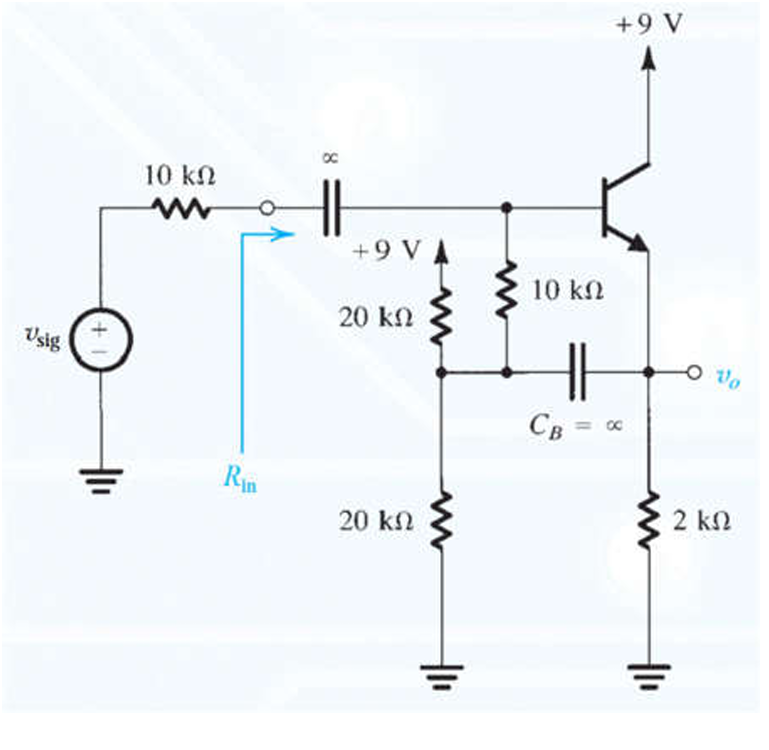
\includegraphics[width=.8\linewidth]{./my-chapters/my-images/Question4/Debai.png}
\end{figure}

\answer{a}{Tìm điểm hoạt động Q của BJT}

\noindent Xét hoạt động chế độ DC cho toàn mạch.

\begin{itemize}[label=-]
	\item Tìm giá trị $V_{BE}$ của BJT trong Multisim
	
	\begin{figure}[H]
		\centering
		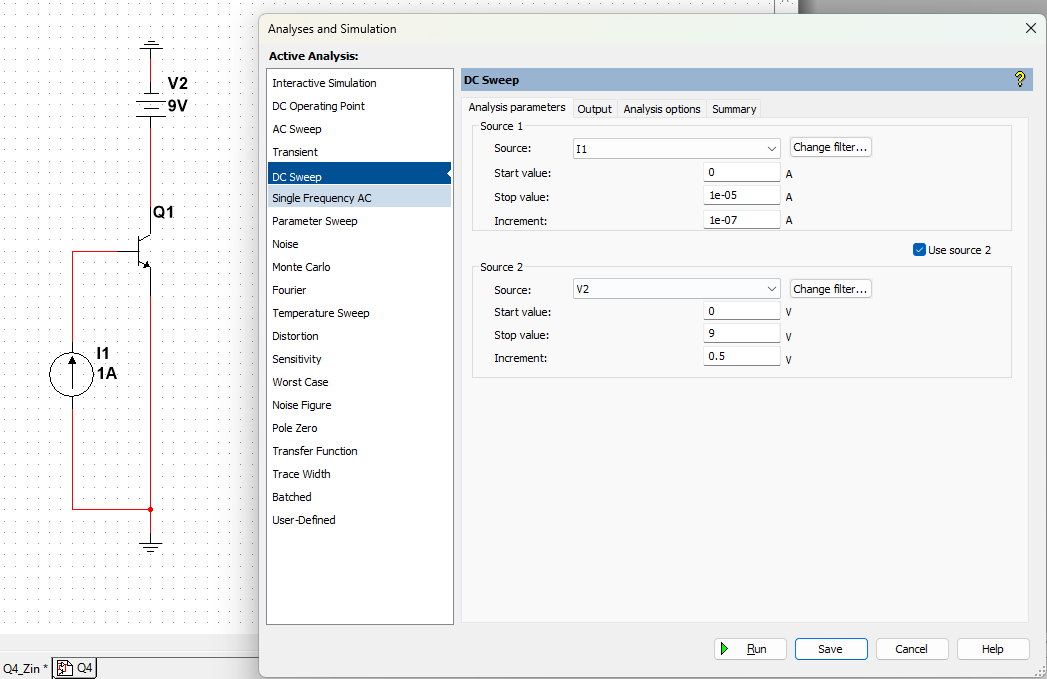
\includegraphics[width=.8\linewidth]{./my-chapters/my-images/Question4/a_doVBE.png}
		\caption{Tìm giá trị $V_{BE}$ của mạch.}
	\end{figure}
	
	Ta sử dụng một chế độ DC Sweep để tìm giá trị $V_{BE}$ dẫn của mạch. Sau khi chạy tool ta có kết quả như sau,
	
	\begin{figure}[H]
		\centering
		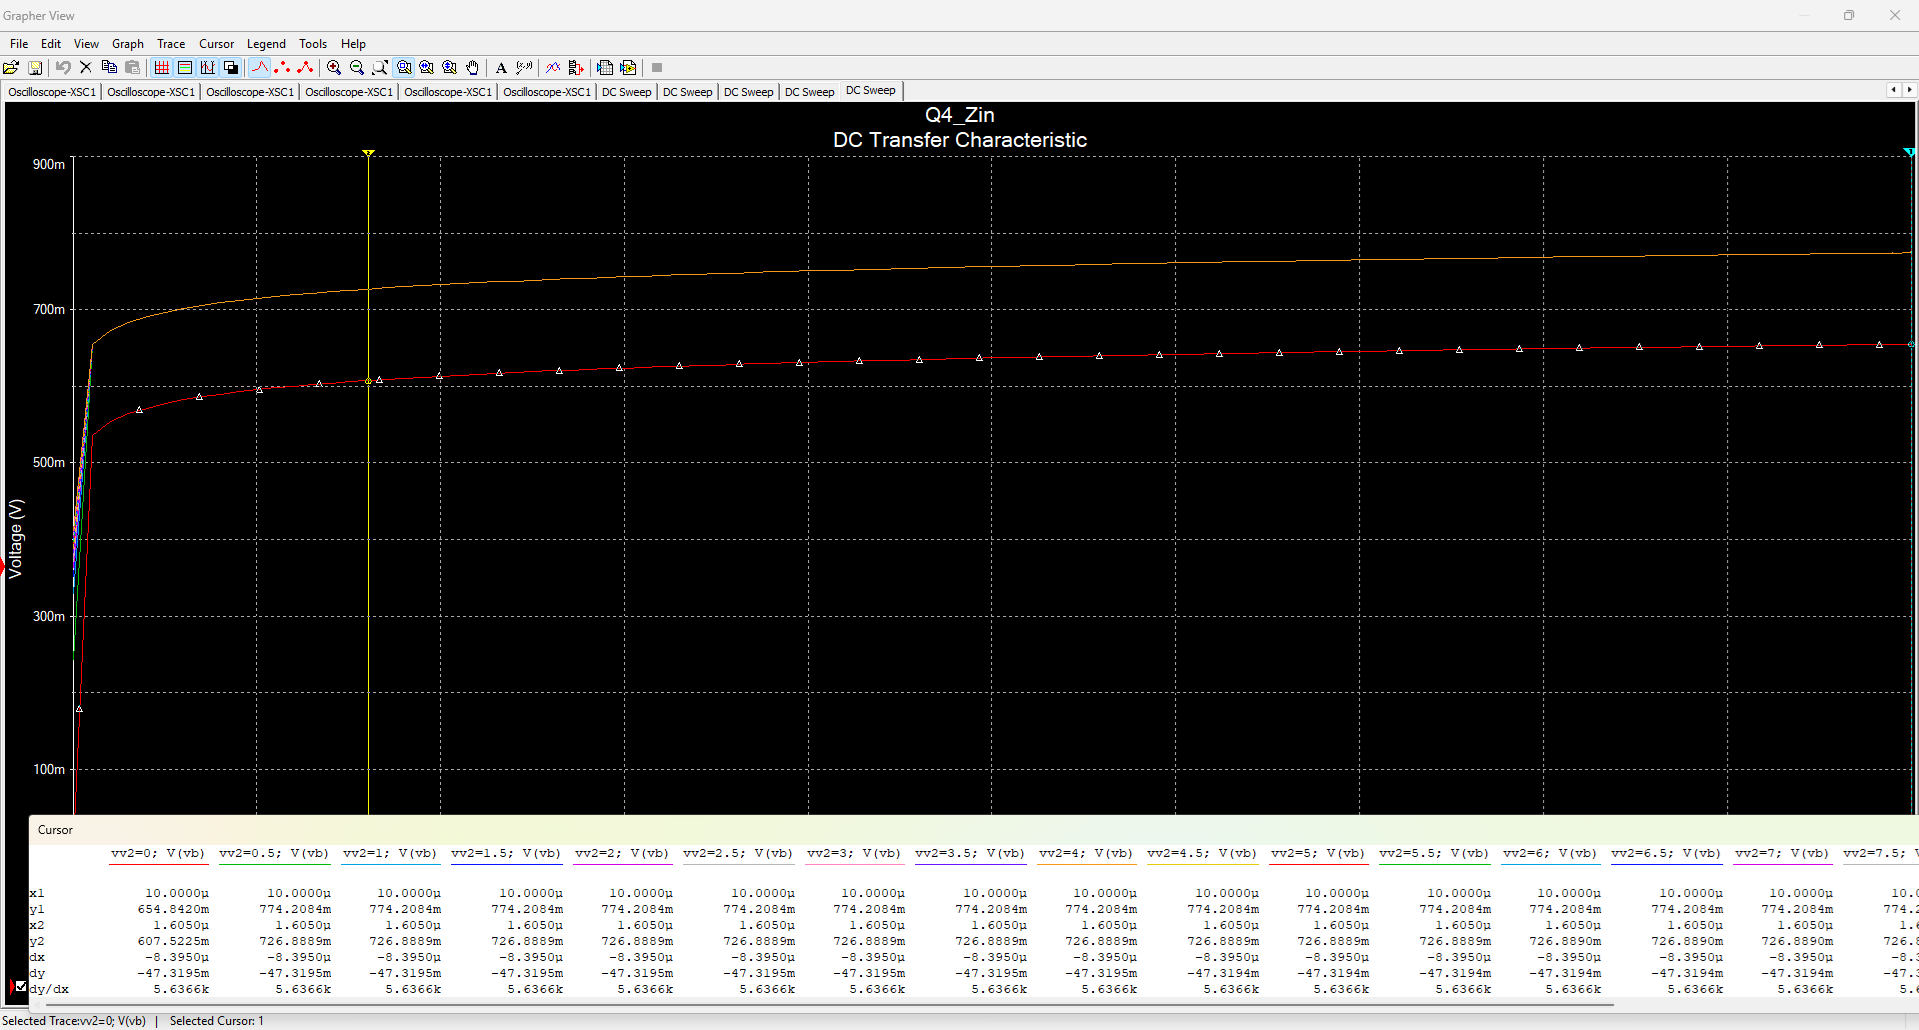
\includegraphics[width=.8\linewidth]{./my-chapters/my-images/Question4/a_timVBE.png}
		\caption{Kết quả sau khi chạy DC Sweep để tìm $V_{BE}$.}
	\end{figure}
	
	Nhìn vậy hình ta thấy được điện áp $V_{BE}$ của BJT dẫn rơi vào tầm $ \approx 0.774\,\text{mA}$. Từ đó, nhóm em chọn $V_{BE} = 0.774\,\text{mA}$ cho câu 4.
	
	\item Tìm giá trị $I_{CQ}$
	
	\begin{figure}[H]
		\centering
		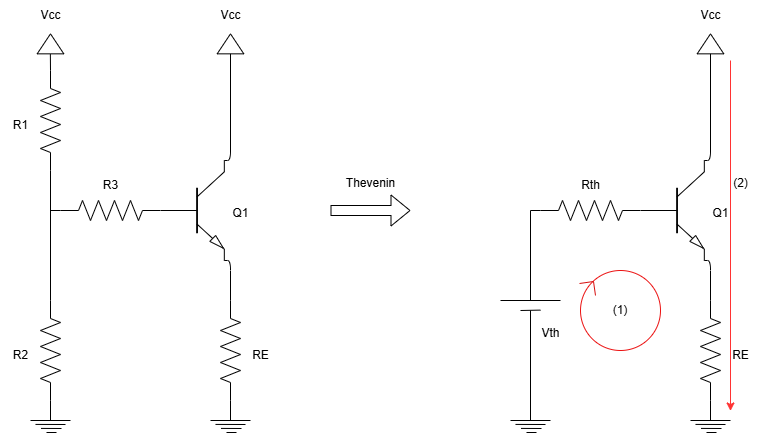
\includegraphics[width=.7\linewidth]{./my-chapters/my-diagrams/Question4/Debai.png}
	\end{figure}
	
	Thevenin ta có:
	\[ R_{th} = R_{3} + R_{1}//R_{2} = 10 + \dfrac{20\times 20}{20 + 20} = 20k\Omega\]
	\[ V_{th} = \dfrac{R_{2}}{R_{1} + R_{2}} V_{cc} = \dfrac{20}{20+20} \times 9 = 4.5V\]
	
	Áp dụng KCL cho vòng (1):
	\[ -V_{th} + I_{B}R_{th} + V_{BE} + I_{E}R_{E} = 0\]
	Ta có: $ I_{E} = (\beta + 1)I_{B} $
	\[\Rightarrow I_{B} = \dfrac{V_{th} - V_{BE}}{R_{th} + (\beta + 1)R_{E}} = \dfrac{4.5 - 0.774}{20 + (100+1)\times 2} = 0.0168\,\text{mA}\]
	Ta có: $I_{C} = \beta I_{B} = 100\times 0.0168\,\text{mA} = 1.68\,\text{mA}$.
	
	\item Tìm giá trị $V_{CEQ}$
	
	Áp dụng KCL cho vòng (2):
	\[ -V_{cc} + V_{CE} + I_{E}R_{E} = 0\]
	Ta có: $I_{C} = \dfrac{\beta}{\beta + 1}I_{E} = \alpha I_{E} \approx I_{E}$
	\[\Rightarrow V_{CE} = V_{cc} - I_{C}R_{E} = 9 - 1.71\times 2 = 5.64V \]
	
	Vậy điểm làm việc Q của tâng 2 là : \finalresult{(I_{CQ}, V_{CEQ}) = (1.68\,\text{\,\text{mA}}, 5.64\,\text{V})}.
	
	\item Kiểm chứng kết quả:
	
	\begin{figure}[H]
		\centering
		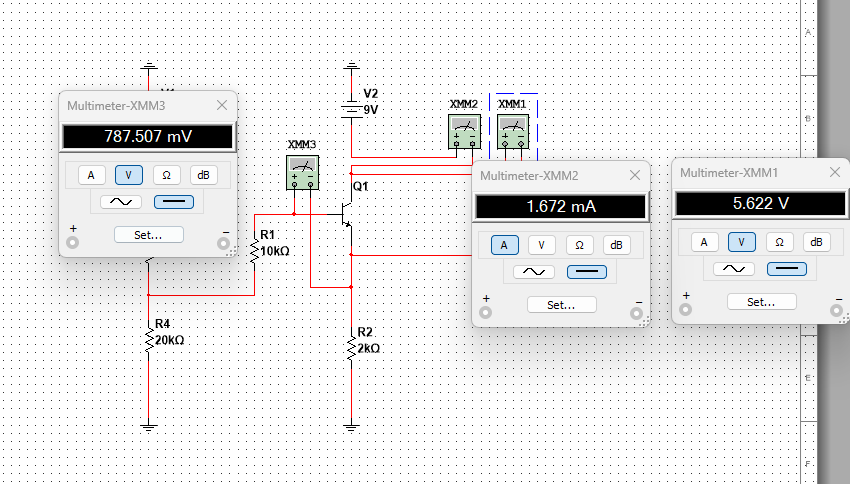
\includegraphics[width=.8\linewidth]{./my-chapters/my-images/Question4/phancucDC_Q.png}
		\caption{Kết quả điểm Q của bài 4.}
	\end{figure}
\end{itemize}

\answer{b}{Đặt $v_{s} = V_{s}\sin \left(\omega t\right)$ vào mạch. Ngõ ra nối với tải $R_{L} = 1k\Omega$. Tìm $A_{vo}$, $G_{v}$, $R_{i}$, $R_{o}$ của mạch.}

\noindent Xét hoạt động chế độ AC cho toàn mạch.

\begin{figure}[H]
	\centering
	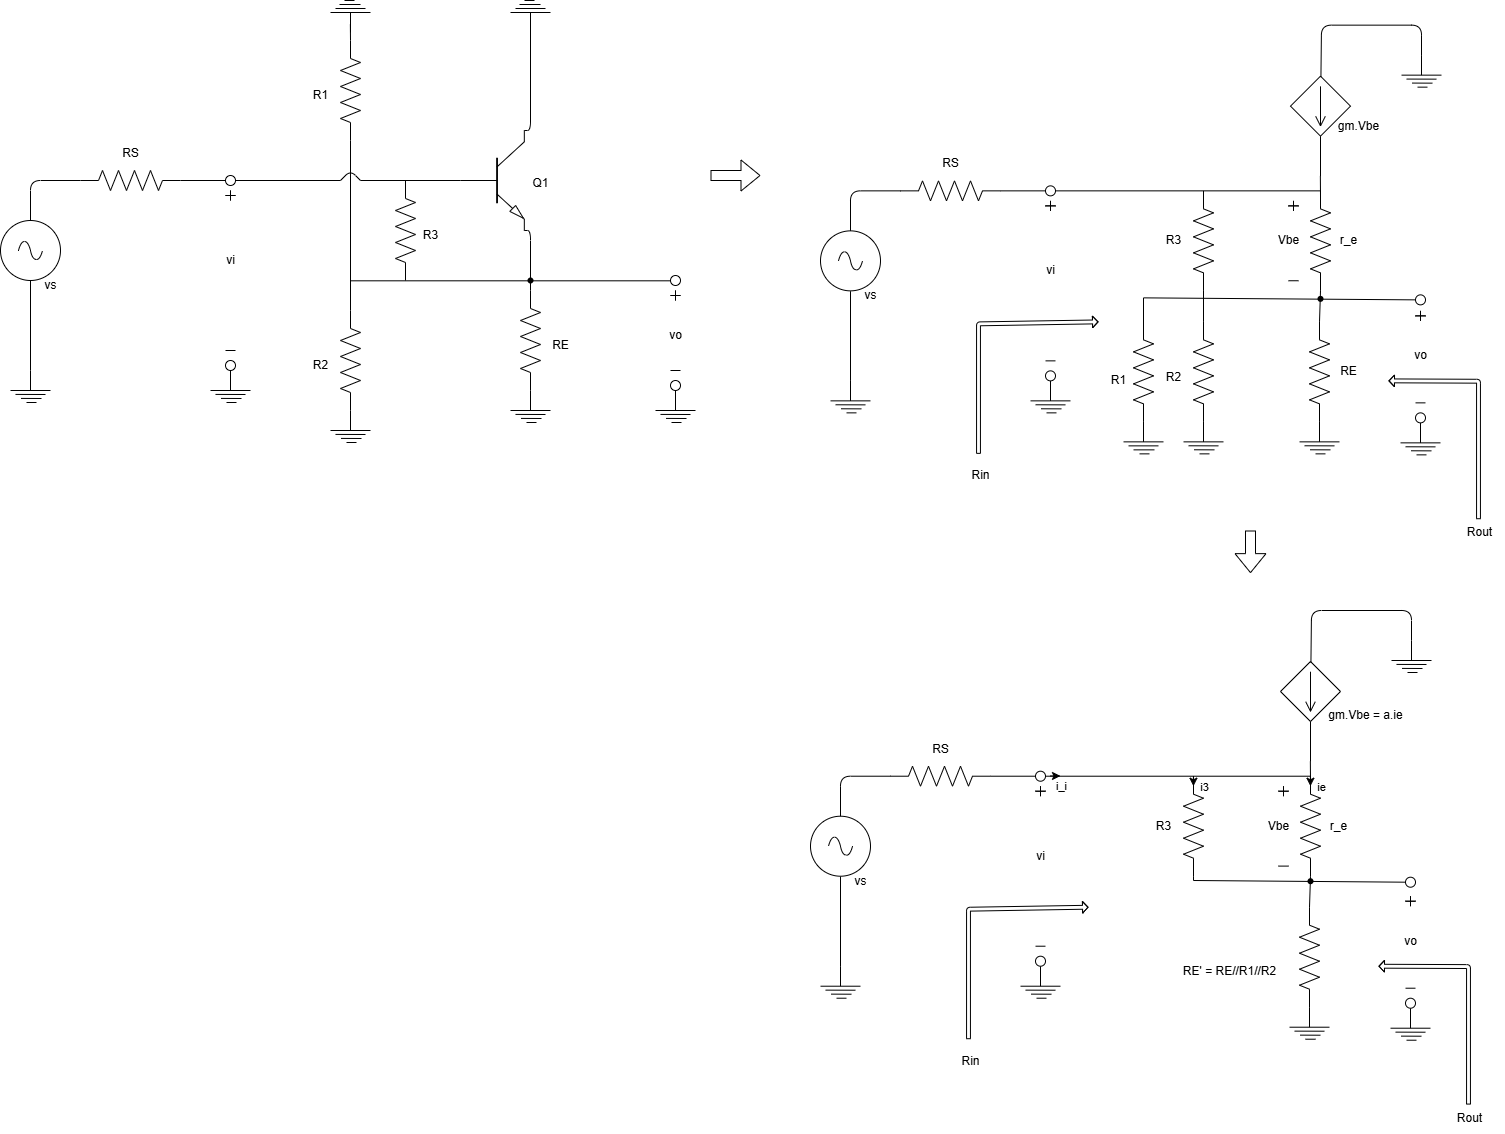
\includegraphics[width=.9\linewidth]{./my-chapters/my-diagrams/Question4/caub_t.png}
\end{figure}

Ta có, 

\begin{itemize}[label=+, leftmargin=2cm]
	\item $R_{E}^{'} = R_{E} // R_{1} // R_{2} \approx 1.6667\,\text{k}\Omega$
	\item $g_{m} = \dfrac{I_{C}}{V_{T}} =  \dfrac{1.68\,\text{m}}{25\,\text{m}} = 67.2mS$
	\item $r_{e} = \dfrac{V_{T}}{I_{E}} = \dfrac{V_{T}}{I_{C}/\alpha} = \dfrac{25\,\text{mV}}{1.68\,\text{mA} / \dfrac{100}{100+1}} \approx 14.7336\,\Omega$
	\item $r_{\pi} = \beta \dfrac{V_{T}}{I_{C}} = 100\times\dfrac{25\,\text{m}}{1.68\,\text{m}} = 1.4881\,\text{k}\Omega$
\end{itemize}

\begin{itemize}[label=-]
	\item Tính giá trị $R_{in}$
	
	Ta có, $R_{in} = \dfrac{v_{i}}{i_{i}}|_{i_{o} = 0}$, đầu tiên ta xét
	
	\begin{itemize}[label=+, leftmargin=1cm]
		\item $i_{i} = i_{3} + i_{e} - \alpha i_{e} $
		
		Trong đó, $i_{3} = \dfrac{i_{e} r_{e}}{R_{3}}$
		
		$\Rightarrow i_{i} = \dfrac{i_{e} r_{e}}{R_{3}} + i_{e}(1-\alpha)$
		\item $v_{i} = v_{be} + v_{o}$
		
		Trong đó, $v_{o} = R_{E}^{'} (i_{3} + i_{e}) = R_{E}^{'} \left( \dfrac{i_{e} r_{e}}{R_{3}} + i_{e} \right)$
	\end{itemize}
	
	$\Rightarrow R_{in} = \dfrac{R_{E}^{'} \left( \dfrac{i_{e} r_{e}}{R_{3}} + i_{e} \right) + i_{e}r_{e}}{\dfrac{i_{e} r_{e}}{R_{3}} + i_{e}(1-\alpha)} = \dfrac{R_{E}^{'} \left( \dfrac{r_{e}}{R_{3}} + 1 \right) + r_{e}}{\dfrac{r_{e}}{R_{3}} + (1-\alpha)} \approx 148.0428 \,\text{k}\Omega$.
	
	$\Rightarrow$ \finalresult{R_{in} = 148.0428\,\text{k}\Omega}.
	
	\item Tính giá trị $R_{out}$
	
	Ta có, $R_{out} = \dfrac{v_{o}}{i_{o}}|_{v_{i} = 0}$
	
	$\Rightarrow R_{out} = R_{E}^{'} // r_{e} // \dfrac{R_{3}}{\beta + 1} = 12.7272\,\Omega$.
	
	$\Rightarrow$ \finalresult{R_{out} = 12.7272\,\Omega}.
	
	\item Tính giá trị $A_{vo}$
	
	Ta có, $A_{vo} = \dfrac{v_{o}}{v_{i}}|_{R_{L} = \infty} = \dfrac{R_{E}^{'} \left( \dfrac{r_{e}}{R_{3}} + 1 \right)}{R_{E}^{'} \left( \dfrac{r_{e}}{R_{3}} + 1 \right) + r_{e}} \approx 0.9913 \,\text{V/V}$.
	
	$\Rightarrow$ \finalresult{A_{vo} = 0.9913 \,\text{V/V}}.
	
	\item Tính giá trị $G_{v}$
	
	ta có, $G_{v} = \dfrac{v_{o}}{v_{s}} = \dfrac{R_{in}}{R_{in} + R_{s}} A_{v} = \dfrac{148.0428}{148.0428 + 10}\times 0.9914 \approx 0.9287 \,\text{V/V}$.
	
	$\Rightarrow$ \finalresult{G_{v} = 0.9287 \,\text{V/V}}. 
	
	\item Kiểm tra kết quả
	
	\begin{figure}[H]
		\centering
		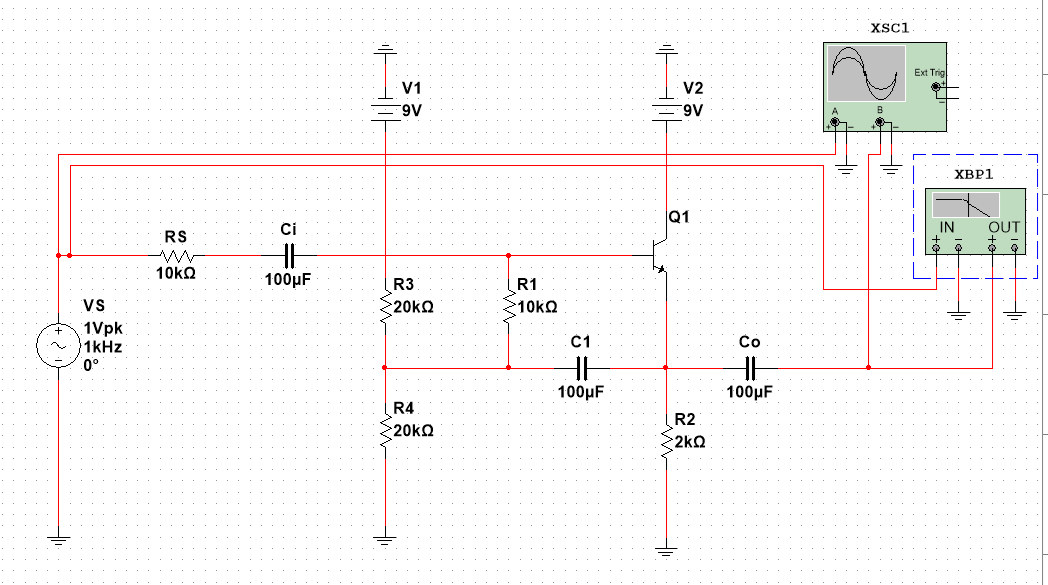
\includegraphics[width=.8\linewidth]{./my-chapters/my-images/Question4/b_GV_test.png}
	\end{figure}
	
	\begin{figure}[H]
		\centering
		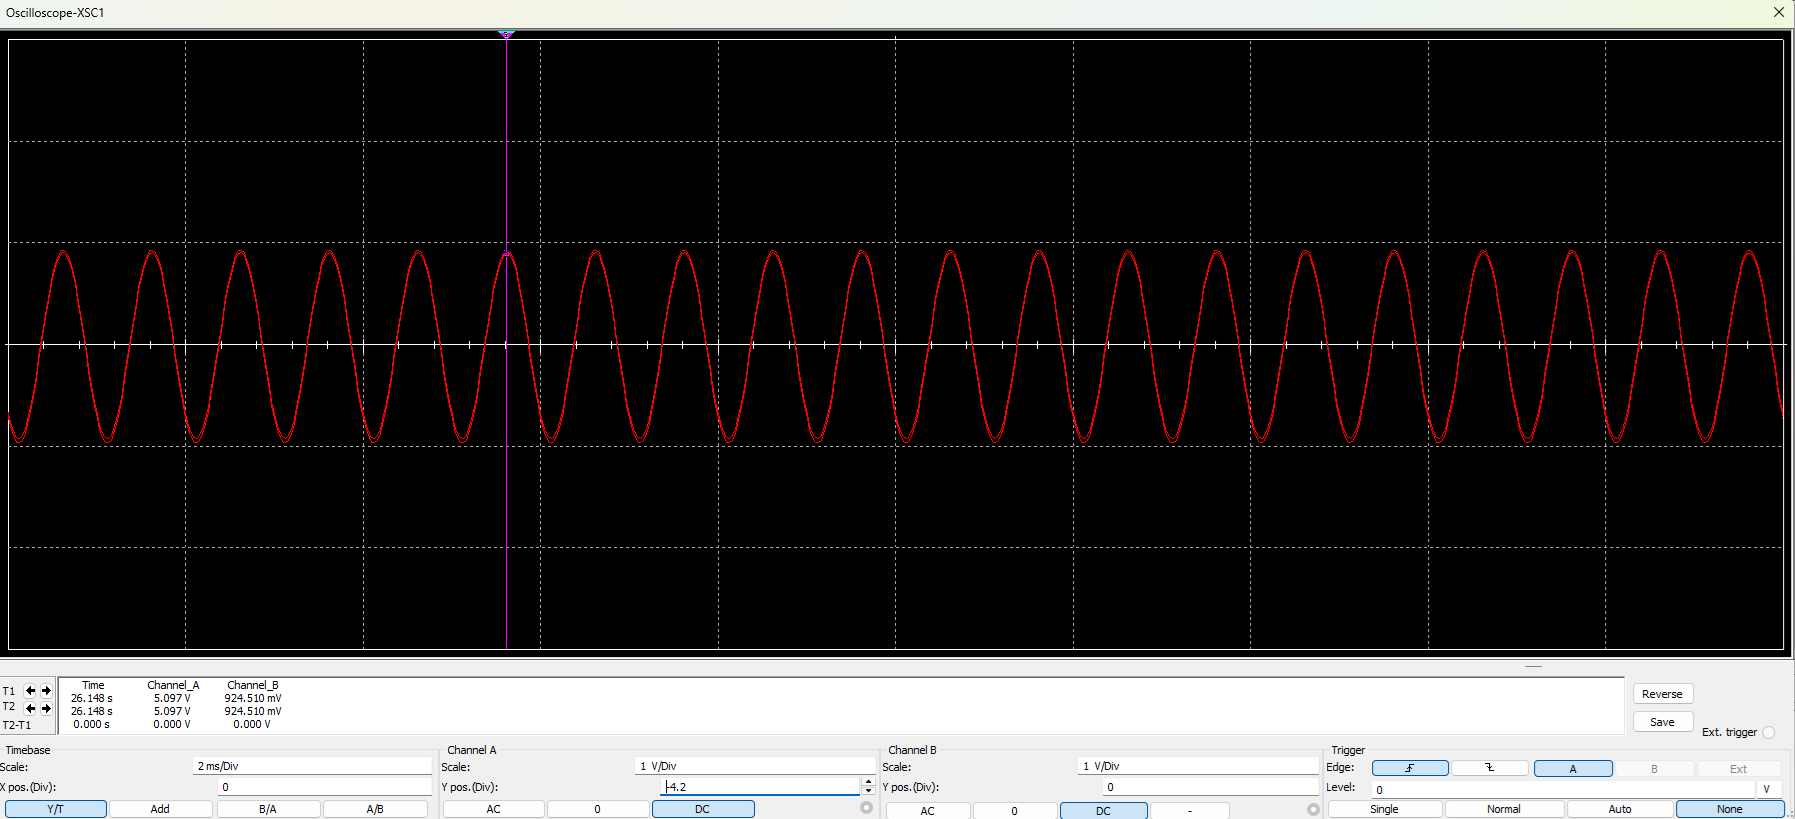
\includegraphics[width=.8\linewidth]{./my-chapters/my-images/Question4/b_Avo_wave.png}
		\caption{Coi dạng sóng ngõ vào và ngõ ra của mạch.}
	\end{figure}
	
	\begin{figure}[H]
		\centering
		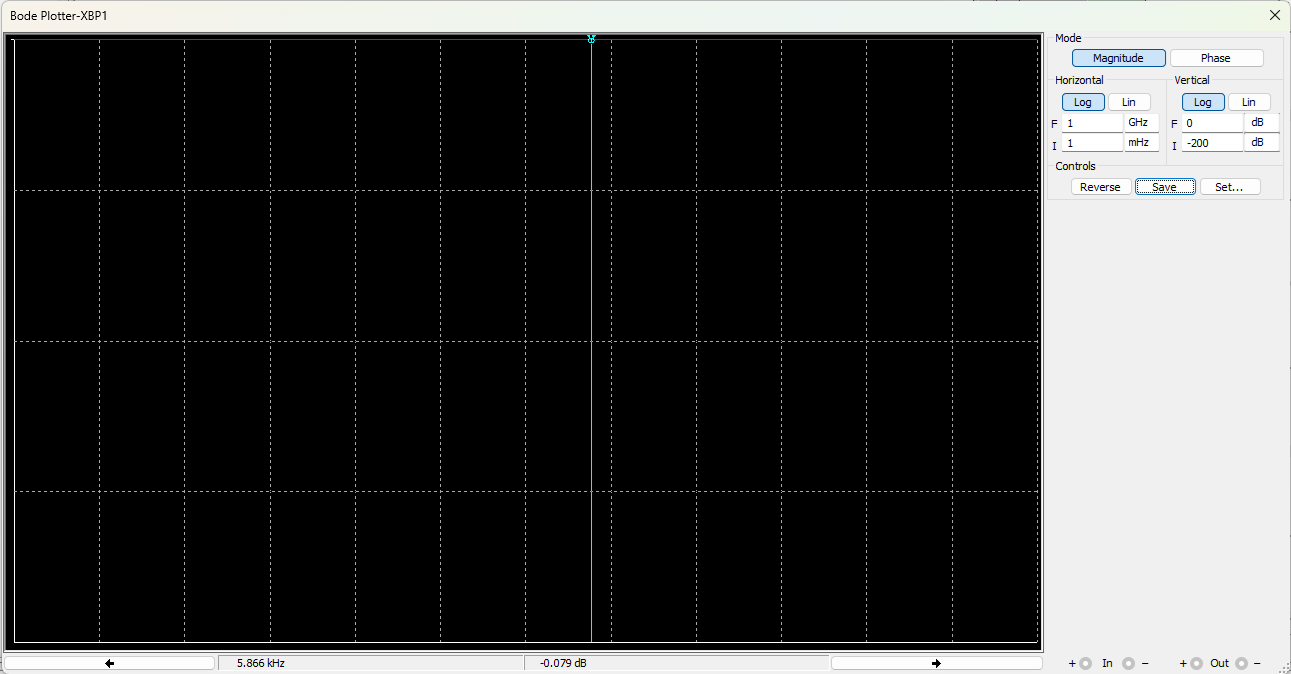
\includegraphics[width=.8\linewidth]{./my-chapters/my-images/Question4/b_Avo_bode.png}
		\caption{Tiến hành đo $A_{vo} = -0.079dB \approx 0.9909$.}
	\end{figure}
	
	\begin{figure}[H]
		\centering
		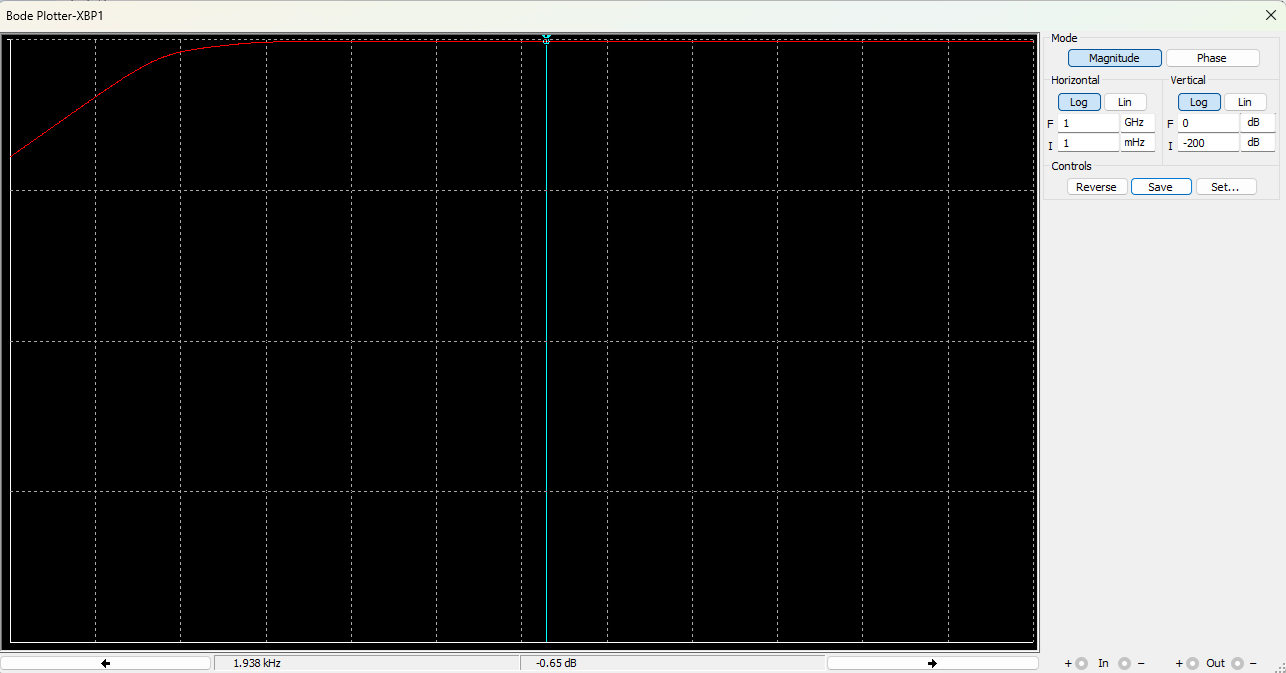
\includegraphics[width=.8\linewidth]{./my-chapters/my-images/Question4/b_GV_bode.png}
		\caption{Tiến hành đo $G_{v} = -0.65dB \approx 0.9279$.}
	\end{figure}
\end{itemize}

\answer{c}{Bỏ tụ $C_{B}$ ra khỏi mạch. Lập lại câu a và b. Từ đó, nêu vai trò của tụ $C_{B}$.}

\begin{figure}[H]
	\centering
	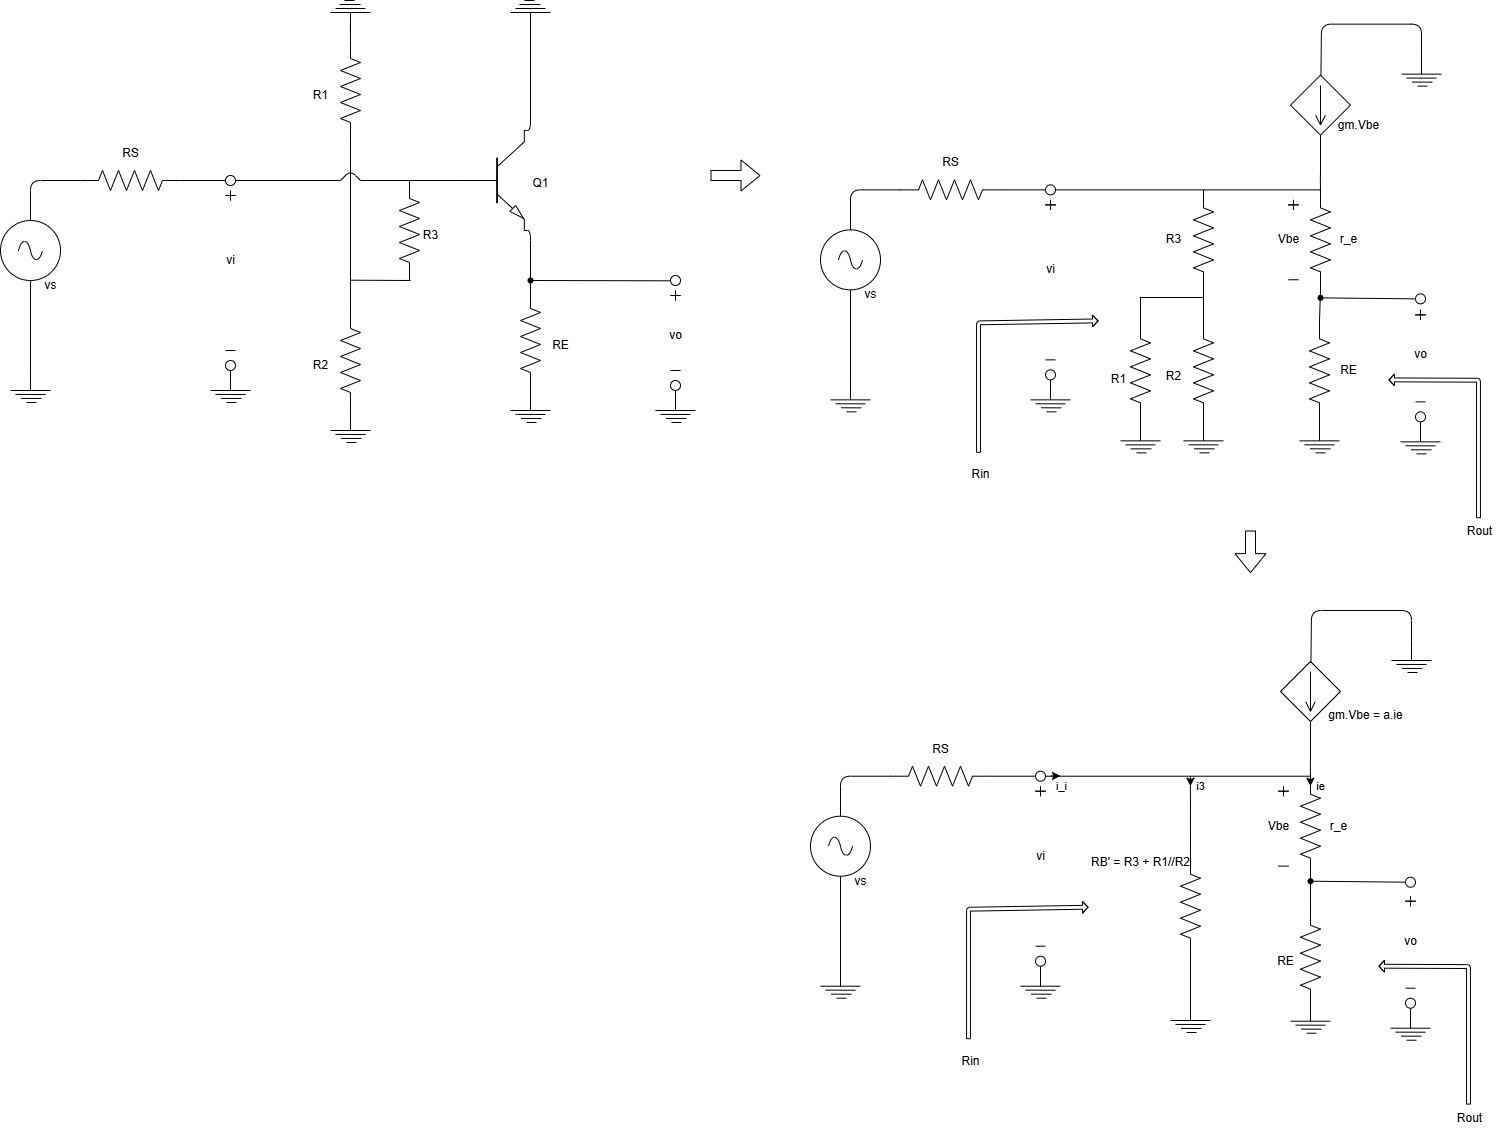
\includegraphics[width=.9\linewidth]{./my-chapters/my-diagrams/Question4/cauc_t.png}
\end{figure}

Ta có, 

\begin{itemize}[label=+, leftmargin=2cm]
	\item $R_{B}^{'} = R_{3} + R_{1} // R_{2} = 20\,\text{k}\Omega$
	\item $g_{m} = \dfrac{I_{C}}{V_{T}} =  \dfrac{1.68\,\text{m}}{25\,\text{m}} = 67.2mS$
	\item $r_{e} = \dfrac{V_{T}}{I_{E}} = \dfrac{V_{T}}{I_{C}/\alpha} = \dfrac{25\,\text{mV}}{1.68\,\text{mA} / \dfrac{100}{100+1}} \approx 14.7336\,\Omega$
	\item $r_{\pi} = \beta \dfrac{V_{T}}{I_{C}} = 100\times\dfrac{25\,\text{m}}{1.68\,\text{m}} = 1.4881\,\text{k}\Omega$
\end{itemize}

\begin{itemize}[label=-]
	\item Tính giá trị $R_{in}$
	
	Ta có, $R_{in} = \dfrac{v_{i}}{i_{i}}|_{i_{o} = 0}$

	\[ \rightarrow R_{in} = R_{B}^{'} // (\beta + 1)(r_{e} + R_{E}) \approx 18.2102\,\text{k}\Omega \]
	$\Rightarrow$ \finalresult{R_{in} = 18.2102\,\text{k}\Omega}.
	
	\item Tính giá trị $R_{out}$
	
	Ta có, $R_{out} = \dfrac{v_{o}}{i_{o}}|_{v_{i} = 0}$ 
	
	\[\rightarrow R_{out} = R_{E} // r_{e} = 14.6259\,\Omega \]
	$\Rightarrow$ \finalresult{R_{out} = 14.6259\,\Omega}.
	
	\item Tính giá trị $A_{vo}$
	
	Ta có, $A_{vo} = \dfrac{v_{o}}{v_{i}}|_{R_{L} = \infty} = \dfrac{R_{E}}{R_{E} + r_{e}} \approx 0.9927\,\text{V/V}$.
	
	$\Rightarrow$ \finalresult{A_{vo} \approx 0.9927\,\text{V/V}}.
	
	\item Tính giá trị $G_{v}$
	
	ta có, $G_{v} = \dfrac{v_{o}}{v_{s}} = \dfrac{R_{in}}{R_{in} + R_{s}} A_{v} = \dfrac{18.2102}{18.2102 + 10}\times 0.9927 \approx 0.6408 \,\text{V/V}$.
	
	$\Rightarrow$ \finalresult{G_{v} = 0.6408 \,\text{V/V}}. 
	
	\item Kiểm tra kết quả
	
	\begin{figure}[H]
		\centering
		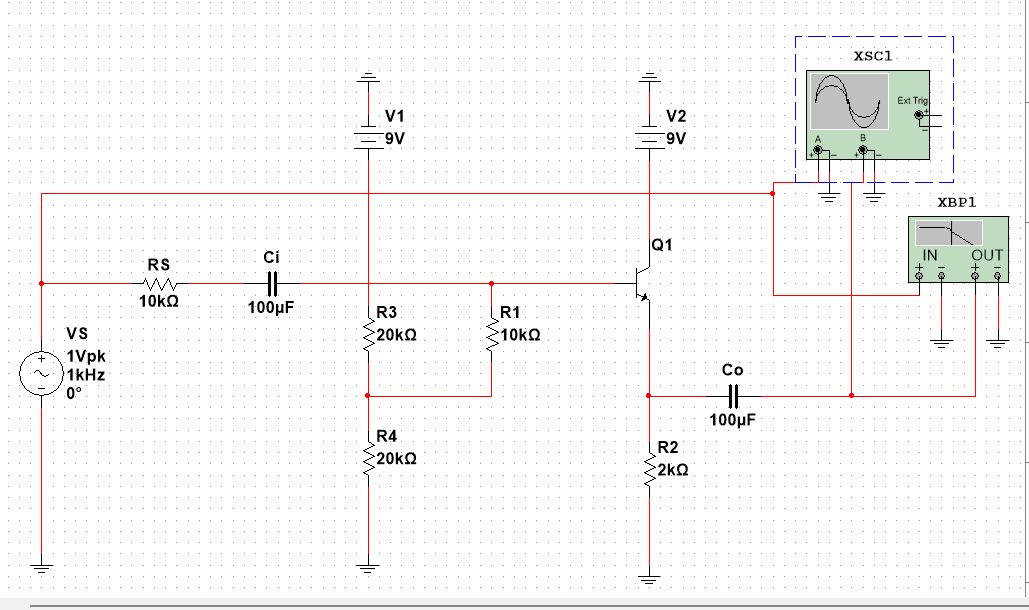
\includegraphics[width=.8\linewidth]{./my-chapters/my-images/Question4/cauc_test.png}
	\end{figure}
	
	\begin{figure}[H]
		\centering
		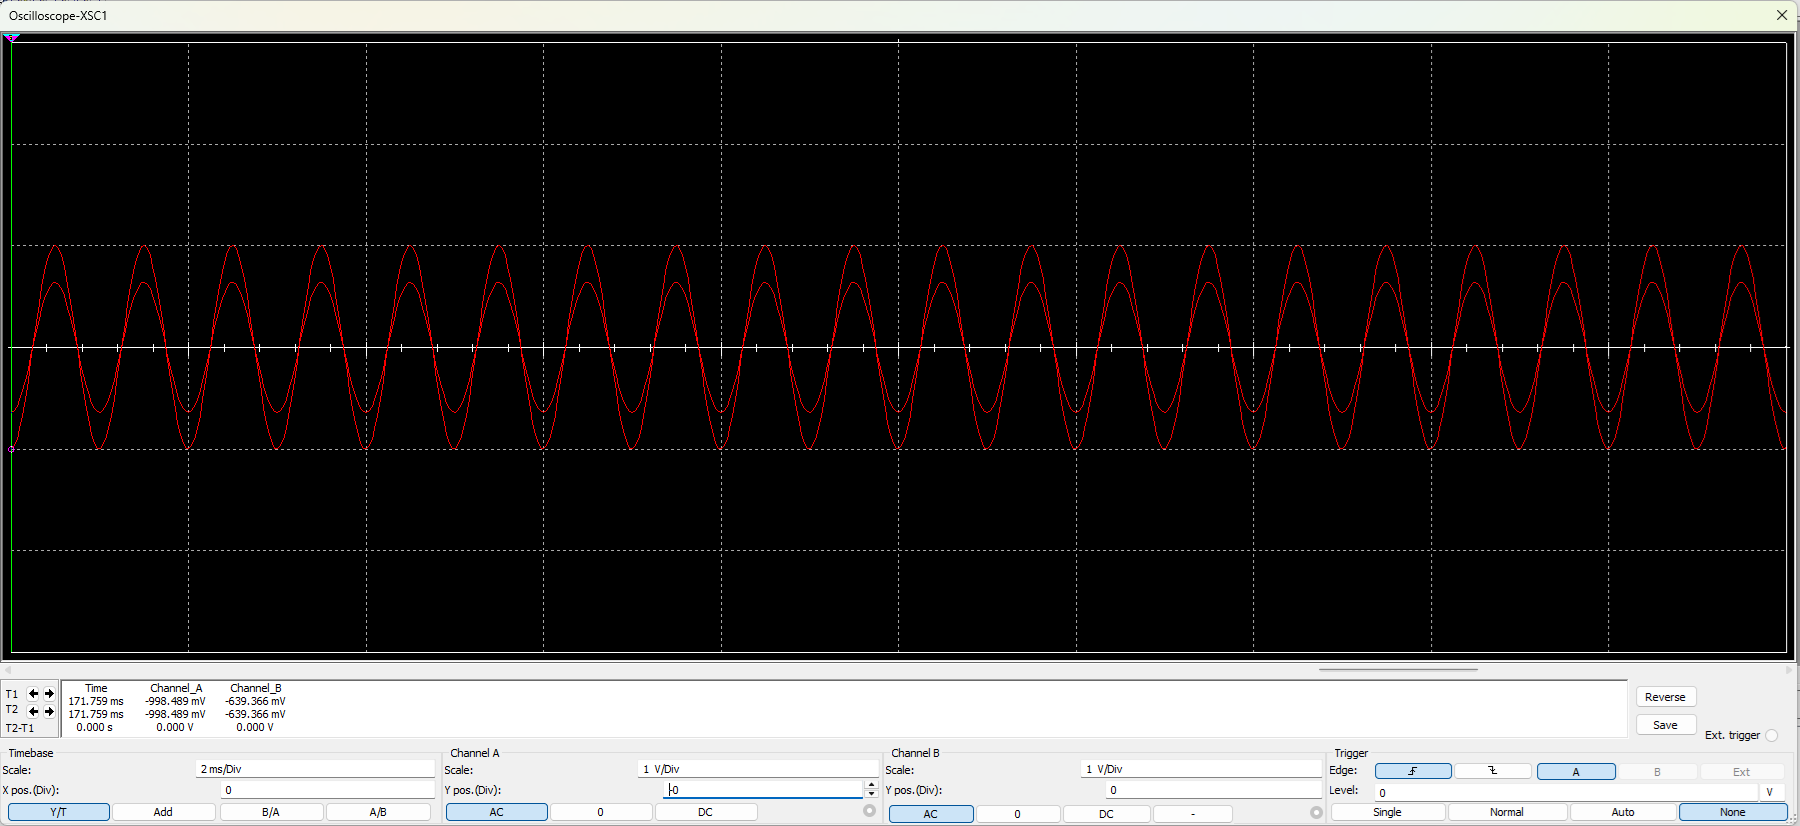
\includegraphics[width=.8\linewidth]{./my-chapters/my-images/Question4/cauc_wave.png}
		\caption{Coi dạng sóng ngõ vào và ngõ ra của mạch.}
	\end{figure}
	
	\begin{figure}[H]
		\centering
		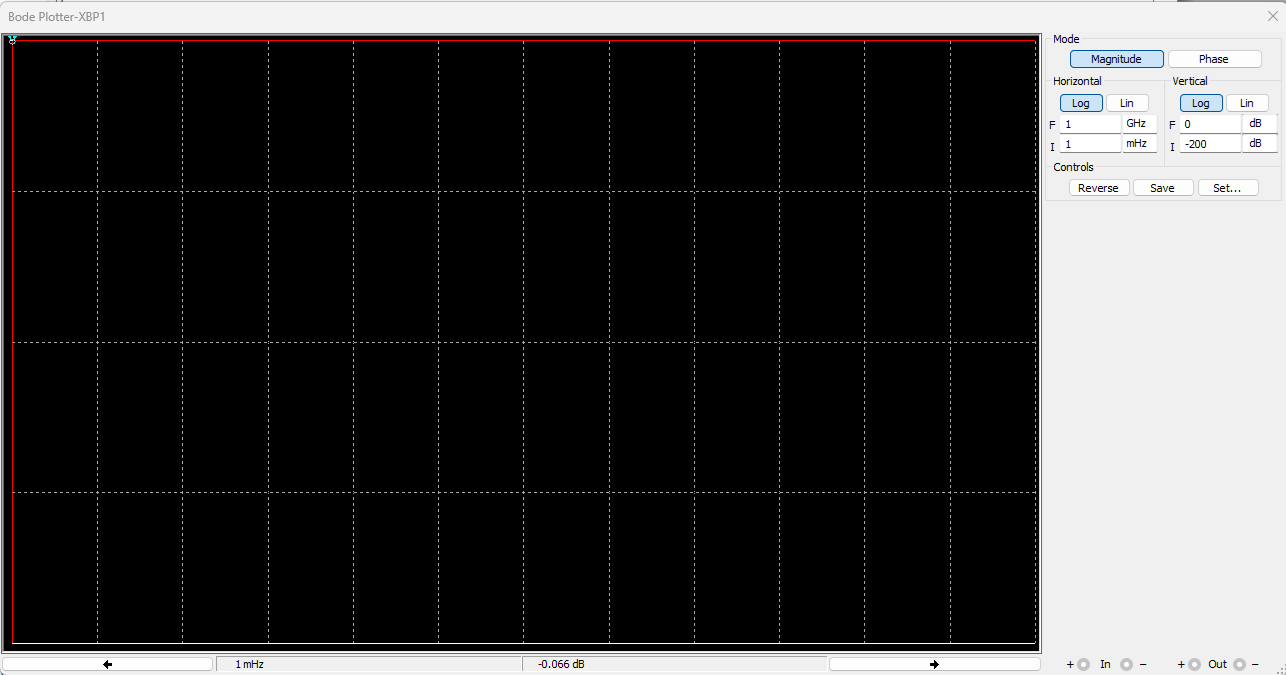
\includegraphics[width=.8\linewidth]{./my-chapters/my-images/Question4/cau_c_bode_avo.png}
		\caption{Tiến hành đo $A_{vo} = -0.066dB \approx 0.9924$.}
	\end{figure}
	
	\begin{figure}[H]
		\centering
		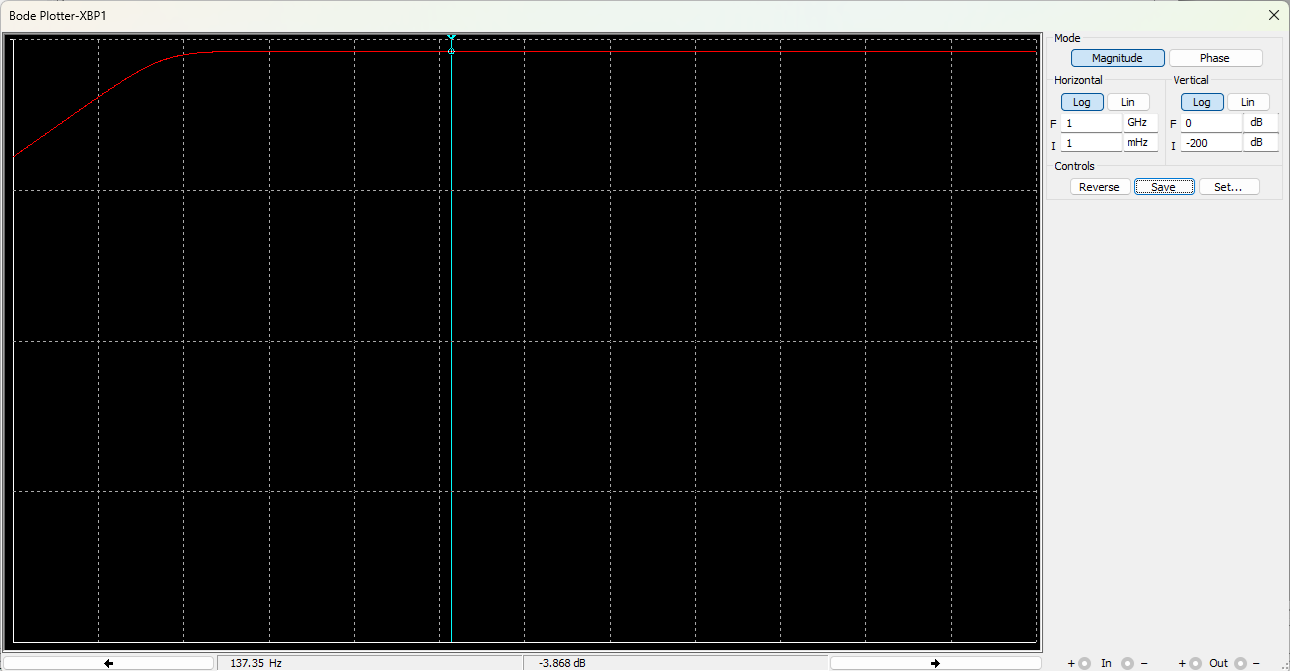
\includegraphics[width=.8\linewidth]{./my-chapters/my-images/Question4/cau_c_bode_gv.png}
		\caption{Tiến hành đo $G_{v} = -3.868dB \approx 0.6406$.}
	\end{figure}
\end{itemize}

\noindent\textbf{Nhận xét}

Mạch trên giống với mạch Bootstrapped Emitter Follower với có một tự $C_{B}$ hồi tiếp dương qua tụ, mạch giúp tăng điện trở đầu vào giúp tăng độ lợi của mạch mà không cần tăng điện trở lên quá cao. Với một trên chỉ cần hồi tiếp về kết hợp một điện trở $R_{1} = 10 \,\text{k}\Omega$ đã có thể tăng $R_{in}$ từ $18.2102\,\text{k}\Omega \rightarrow 148.0428 \,\text{k}\Omega$ có nghĩa là tăng lên đến tầm $8$, và tăng độ lợi $G_{v}$ từ $0.6408 \rightarrow 0.9287$.